\chapter[问候]{问候}
%\chapter[短标题显示在页面]{长标题显示在目录}

% {\small\textit{
% \quad Sors de l'enfance, ami réveille toi!\newline
% \quad \quad —Jean Jacques Rousseau.}
% \footnote{Ekster el infaneco,amiko veku!}
% \\}

\emoji{x_sena}
% \begin{figure}[h]
% 
\includegraphics{pngs/x_sena.png}
% \label{x_sena}
% \end{figure}

欢迎来到Lein的课程!

大家好, 我是学生紫苑. 现在17岁,在上高二.

\emoji{l_sena}

Soonoyun [so:nɔjɯn]! 我叫Lein,是你的老师. 我也是Arbazard中学的学生.
\footnote{这几位女生是``紫苑之书''中的主人公,Nias Avelantis制作了立绘(还包含以后会介绍的Alia和Arshe).感谢他的贡献}

我本来不该说汉语的,但是编辑叫我说我就说吧. :)

\emoji{x_knoos}

那个,你说的第一个词是啥? 额... soonoyun ?

还有Arbazard又是哪?我在世界地图上没找到.

\emoji{l_rana}

Soonoyun 意思是``你好''. 它可以指代早上好,中午好和晚上好.有用吧?
Arbazard是Atolas的一个国家,而Atolas是我居住的星球. 我们国家通行的语言就是Arka.

\emoji{x_naki}

Arka不是地球上的语言吧?怪不得我没见过这些字母.
\begin{figure}[H]
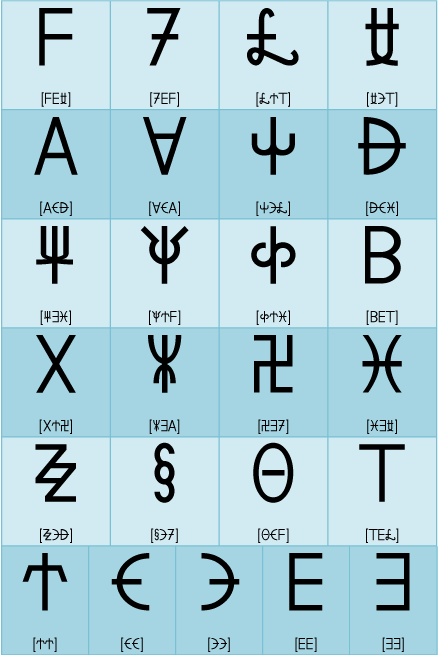
\includegraphics[width=0.5\textwidth]{ARKA/klandi.png}
\end{figure}
\emoji{l_deyu}

这些字母是幻字的大写字母.
20个是辅音,5个是元音,总共有25个.
在Arka中,幻字被叫做hacm.

\emoji{x_lek}

这也忒难记了吧!

我可能记得住E 和 F, but...

\emoji{l_ket}

其实, 我们很少用大写字母,你只要记住这些小写字母就行了.
\begin{figure}[H]
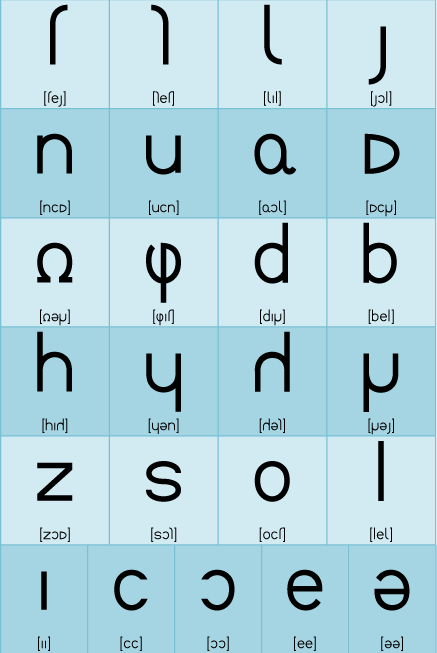
\includegraphics[width=0.5\textwidth]{ARKA/lemal.png}
\end{figure}
\emoji{x_tisse}

这样啊,那说不定能行.所有字母都只有一画,有些字母还和拉丁字母很像.
幻字来自别的世界,但某种程度上还真是相似啊.

\emoji{l_rana}

你发现了奇妙的东西呢.不过关于字母的文章现在对你来说还太难.

\emoji{x_lo}

小写字母虽说简单,但我还是要花点功夫记.现在嘛,我要用拉丁字母转写Arka.
在我熟悉字母表之前,我还是先看这个语言的转写版凑合.
\begin{figure}[H]
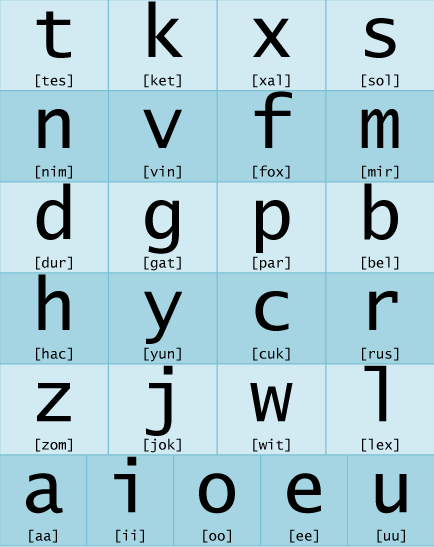
\includegraphics[width=0.5\textwidth]{ARKA/tenxa.png}
\end{figure}
\emoji{x_lo}

转写的Arka大部分都还行.就是``x''和``c''发音有些奇怪.``x''发[ʃ](像``shop''里的``sh''),``c''是卷舌的 R (像西班牙词``burro''里的``rr'').

So, ``c''是齿槽颤音[r], whereas ``r''是齿槽近音[ɹ].

其他的字母...? ``y'' ([j])像"yes."的``y'', ``j'' ([ʒ])像``vision''的``s''.``h''([h])像``happy''里的``h'', ``w'' ([w])像``wise''的``w''.

\emoji{l_rana}

熟悉幻字的时候就用拉丁转写吧. ``tx'' ([tʃ])像  ``church''的``ch'',``ts''发``cats''的``ts''.

幻字是专门书写Arka的,所以用来写Arka就很有效.一步一步来嘛.

很多字母都相互对称;我小时候就经常把``tes''混成``ket''.长大了就分的清了,就像你区分``d''和``b''一样.

\emoji{x_sena}

看来我应该一步一步来,多动笔写写.
不管咋样,我该练练转写啦.\textbf{``x''发``shop''的``sh'', ``c''发西班牙语``burro''的``rr''.}
说干就干!

%"([a-z]+)"
%``$1''


